\chapterauthor{Piotr Korycki, Krzysztof Kępa}
\chapter[Uczenie maszynowe \ldots]{Uczenie maszynowe w klasyfikacji emisji urządzeń radiowych}
\label{rffp} % Always give a unique label
% use \chaptermark{}
% to alter or adjust the chapter heading in the running head

\thispagestyle{empty}
\vspace{-8mm} {\large Piotr Korycki, Krzysztof Kępa} \vspace{8mm}

\section{Wprowadzenie}
Identyfikująca klasyfikacja emisji urządzeń radiowych (Radio Frequency Fingerprinting) to forma analizy sygnału radiowego oparta na rejestracji i analizie niedoskonałości w sygnale urządzeń radiowych. Każde urządzenie telekomunikacyjne opiera się na module transmisyjnym, który odpowiada za konwersję sygnału cyfrowego na analogowy w postaci emitowanych fal radiowych. Urządzenia analogowe odpowiedzialne za generowanie sygnału radiowego posiadają unikalne dla siebie niedoskonałości wynikające z artefaktów produkcyjnych, np. nieliniowość wzmacniacza, które zgodnie z dotychczasowymi badaniami \cite{rf_fingerprinting_sciencedirect} są możliwe do zarejestrowania. Co bardziej istotne, na ich podstawie można określić unikalną charakterystykę toru nadawczego, która pozostanie na stałe przypisana do konkretnej jednostki. Do najważniejszych zastosowań klasyfikacji sygnałów radiowych można zakwalifikować:
\begin{enumerate}
    \item Autoryzacja urządzeń sieciowych. Możliwość klasyfikacji modułów transmisyjnych, zaproponowana m.in. przez autorów opracowań \cite{sankhe2019oracle} i \cite{kaur2020rf}, otwiera przed przemysłem telekomunikacyjnym całkowicie nowy rozdział bezpieczeństwa sieci, w którym autoryzacja urządzeń sieciowych odbywa się nie tylko w warstwie logicznej, ale również w warstwie fizycznej, z całkowitym pominięciem takich aspektów anonimowości jak dowolne protokoły szyfrowania.
    \item Deanonimizacja urządzeń. W informatyce śledczej istnieje potrzeba nabycia zdolności do klasyfikacji urządzeń bezprzewodowych. Deanonimizacja fizycznych nadajników może posłużyć do weryfikacji czy dane urządzenie było odpowiedzialne za przeprowadzony atak (np. WiFi Deauthentication) Możliwość odróżniania nadajników w komunikacji bezprzewodowej w tym m.in. stanowiących coraz większe zagrożenie dla bezpieczeństwa cywilnego bezzałogowych systemów latających, badanych w opracowaniu \cite{soltani2021RF}, czy klasyfikacja telefonów komórkowych na bazie ich emisji w technologiach Bluetooth, LTE, 5G, czy Wi-Fi udostępni organom kontrolującym i~regulatorom krajowym niedostępny dotąd poziom przeprowadzania rozpoznania elektronicznego.
    \item Automatyczna detekcję modulacji. Systemy telekomunikacyjne stosują w~transmisji różne rodzaje modulacji sygnału, które zmieniają się w zależności od możliwości punktu dostępowego (Access Point) oraz jakości odbieranych danych. W sytuacji, w której sygnał jest silnie stłumiony, nadajnik jest zmuszony do zmiany na modulację niższego rzędu. Ze względu na to, że są to systemy o wysokiej wydajności i przepustowości, przyspieszenie czasu rozpoznawania odbieranej modulacji, może pozytywnie wpłynąć na rozwój technologii bezprzewodowych. Opis metod realizujących detekcję modulacji znajduje się m.in. w pracach \cite{8362982} i \cite{wang2016distributed}.
\end{enumerate}

Choć możliwe do zarejestrowania odchylenia (zniekształcenia) były znane badaczom od początku rozwoju technologii bezprzewodowych, to istotny przełom w dziedzinie analizy niedoskonałości nastąpił wraz z dynamicznym rozwojem sztucznej inteligencji, w tym przede wszystkim dzięki metodom uczenia nadzorowanego, które w przeciwieństwie do stosowanego wcześniej algorytmu wektorów wspierających, będącego algorytmem uczenia bez nadzoru, potrafią wykorzystać ciągle zwiększające się możliwości obliczeniowe i skalować się wraz z rozmiarem dostępnych danych.

Do najważniejszych wyzwań stojących przed rozwojem technologii klasyfikacji sygnałów radiowych, przywołanych w artykule \cite{soltani2021RF} można zaliczyć:
\begin{enumerate}
    \item Wpływ sprzętu odbiorczego, opisany w pracy \cite{yang2024mitigatingreceiverimpactradio}. Podobnie jak urządzenia nadawcze wprowadzają unikalne zniekształcenia, tak sprzęt pomiarowy, który rejestruje i przetwarza te emisje w celu klasyfikacji, może wpływać na poprawność zastosowanej metody. W szczególności szumy fazowe, przesunięcia zegara, zniekształcenia filtrów, odchylenia IQ itp. wprowadzone przez urządzenie odbiorcze mogą stworzyć własny, unikalny "odcisk palca", przekształcając dane nadajnika tak, że mogą one wyglądać jak pochodzące od fałszywego lub niezidentyfikowanego emitera.
    \item Badanie podatności systemów autoryzacji opartych na klasyfikacji sygnałów radiowych. Zdalna komunikacja nadajników bezprzewodowych, czasem na dużą odległość, czyni je podatnymi na ataki takie jak fałszowanie tożsamości. Przykładami takich zagrożeń są ataki typu DoS (Denial of Service), podszywanie się, czy kradzież pasma. Ważnym aspektem rozwoju metod klasyfikacji sygnałów radiowych jest fakt, że pasywni odbiorcy sygnału mogą budować własne zestawy danych dotyczące emisji specyficznych nadajników w celu stworzenia specjalizowanych poznawczych systemów klasyfikacji. Istotnym problemem badawczym, mającym wpływ na zwiększenie bezpieczeństwa sieci bezprzewodowych jest opracowanie technik, które programowo zmodyfikują lub zakłócą zestaw cech nadajnika w taki sposób, aby nie mógł on być wyodrębniony przez pasywnych odbiorców, lub w~systemie autoryzacji zostałby zaklasyfikowane jako urządzenie, pod które się podszywa.
    \item Różnica między warunkami kontrolowanymi a rzeczywistością. Ważnym zagadnieniem jest realizm generowanych lub syntetycznych danych. Uogólnienie modeli głębokiego uczenia na rzeczywiste emisje radiowe po ich trenowaniu na danych syntetycznych jest trudne do osiągnięcia. Ta luka w~zdolnościach, opisana w pracy \cite{O_Shea_2018}, wynika z~założeń dotyczących niedoskonałości sprzętu nadawczego i kanału zaniku, które są przyjmowane podczas generowania zestawu danych syntetycznych (np. emitowanych za pomocą platformy USRP), w kontraście do rzeczywistych efektów sprzętowych i~środowiskowych.
    \item Dokładność i skalowalność modeli. Większość dotychczasowych badań została przeprowadzona w warunkach kontrolowanego szumu oraz na stosunkowo niewielkiej liczbie testowanych urządzeń. W praktycznych zastosowaniach systemów opartych o klasyfikację sygnałów radiowych dokładność i~liczba rejestrowanych cech powinna być zostać wyraźnie zwiększona.
\end{enumerate}

\subsubsection*{Cel projektu}

Celem tego projektu jest opracowanie metody automatycznej akwizycji sygnału z~urządzeń transmisyjnych działających w standardzie IEEE 802.11n oraz przygotowania algorytmów i modeli służących do przetwarzania i analizy pozyskanych danych.

\subsubsection*{Zakres pracy}

Zakres pracy obejmuje:
\begin{enumerate}
    \item Zdefiniowanie powtarzalnego schematu doświadczenia, w którym przy dostępnej infrastrukturze będą przeprowadzane pomiary.
    \item Badanie możliwości wymuszenia powtarzalnych transmisji na poszczególnych urządzeniach komercyjnych.
    \item Implementacja procedur sterowania urządzeniami pomiarowymi oraz transferu danych pomiarowych.
    \item Zaprojektowanie algorytmów wstępnej obróbki sygnału w celu  normalizacji jego parametrów.
    \item Opracowanie i demonstracja modeli służących do klasyfikacji urządzeń na podstawie niedoskonałości w amplitudzie oraz fazie emitowanego sygnału.
\end{enumerate}


\section{Przegląd literatury}
Wśród dotychczas badanych podejść do klasyfikacji sygnału urządzeń radiowych możena wyróżnić podejścia bazujące na metodach uczenia bez nadzoru oraz metody uczenia maszynowego wymienione w artykule \cite{rf_fingerprinting_sciencedirect}.
\subsection{Oracle}
W projekcie ORACLE (Optimized Radio clAssification through Convolutional neuraL
nEtworks) \cite{sankhe2019oracle} autorzy przedstawili system identyfikacji urządzeń oparty na klasyfikacji sygnału, bazującym na niedoskonałościach w próbkach IQ. Praca ta przedstawia jedne z najlepszych dotychczas osiągniętych wyników, w których autorzy demonstrują dokładność klasyfikacji wynoszącą do 99\% na ponad 100 komercyjnych urządzeniach Wi-Fi. Na podstawie analizy sygnału nadajników USRP X310\footnote{~\url{https://www.ettus.com/all-products/x310-kit}} ORACLE demonstruje wpływ na klasyfikację celowo ustalonych niedoskonałości w generowanym sygnale.

W kontekście badania wpływu nieprawidłowości sprzętowych autorzy skupiają się na niezbilansowanym IQ (In-phase Quadrature) i przesunięciu DC (Direct Current offset). Do generowania pakietów zgodnych z normą IEEE 802.11a autorzy projektu wykorzystali pakiet MATLAB Communications System Toolbox\footnote{~\url{https://www.mathworks.com/products/communications.html}}, a~także opracowaną w projekcie DARPA \cite{darpa_spectrum_2017} bazę danych, która zawierała surowe próbki IQ zebrane z 140 urządzeń, w tym telefonów, tabletów, laptopów i dronów pochodzących od 122 producentów. Przedstawiona w tej pracy metoda klasyfikacji opiera się na modelu konwolucyjnej sieci neuronowej.

\subsection{Bezzałogowe aparaty latające}
Autorzy pracy \cite{soltani2021RF} zaproponowali metodę identyfikacji radiowej dla dronów, opartą na klasyfikatorze składającym się z wielu modeli. Metoda ta łączy wyniki kilku głębokich sieci neuronowych, z których każda jest trenowana na innej części zbioru treningowego. W badaniach zebrano dane od 7 identycznych dronów DJI M100 za pomocą odbiornika USRP X310 z modułem UBX 160\footnote{~\url{https://www.ettus.com/all-products/ubx160}}, pracującego w komorze bezodbiciowej (ang. anechoic chamber).

Sygnał urządzeń został zarejestrowany w różnych odległościach pomiędzy dronem a odbiornikiem, z~czego dla każdej jednostki i każdej odległości zebrano cztery dwusekundowe serie sygnałów, z których każda zawierała około 140 sekwencji danych. Do klasyfikacji zastosowano zmodyfikowane wersje sieci AlexNet (AlexNet1D) \cite{NIPS2012_c399862d} oraz ResNet50 (ResNet1D) \cite{he2015deepresiduallearningimage}. Sieć AlexNet1D składa się z~pięciu bloków, z których każdy zawiera dwie jednowymiarowe warstwy konwolucyjne ze 128 filtrami o rozmiarach odpowiednio 7 i 5, a następnie warstwę MaxPooling. Na szczycie sieci znajdują się dwie w pełni połączone warstwy o~rozmiarach odpowiednio 256 i 128.

Badanie to jako pierwsze pokazuje wpływ unoszenia się dronów w powietrzu na dokładność metod identyfikacji opartych na głębokim uczeniu. Gdy sieć jest trenowana na wszystkich czterech seriach danych, współczynnik klasyfikacji jest bliski 90\%; jednak gdy sieć jest trenowana na trzech pierwszych seriach, a~testowana na czwartej, dokładność obu architektur spada do 50\%. Spadek ten pokazuje wpływ ciągłej zmienności kanału oraz niewielkich ruchów drona podczas unoszenia się. Autorom projektu udało się zminimalizować ten efekt i osiągnąć współczynnik klasyfikacji równy 91\%.

\subsection{Paradis}
%10.1145/1409944.1409959
Projekt Paradis (Passive RAdiometric Device Identification System) \cite{10.1145/1409944.1409959} to model wykorzystujący jednocześnie wiele charakterystyk sygnału, w tym:
\begin{enumerate}
    \item Przesunięcie częstotliwości.
    \item Stopień korelacji preambuły synchronizacji mierzonego sygnału z sygnałem idealnym.
    \item Niezbilansowanie IQ.
    \item Błąd amplitudy.
    \item Błąd fazy.
\end{enumerate}
Metody uczenia, wykorzystane w tym modelu to klasyfikator oparty na algorytmie SVM, który przyjmuje pojedynczą sygnaturę radiometryczną jako dane wejściowe i zwraca najbardziej prawdopodobną etykietę źródła wraz z~miarą pewności oraz klasyfikator oparty na algorytmie k-najbliższych sąsiadów (k-NN), który dla każdej karty sieciowej posiada jeden klasyfikator, obliczający podobieństwo między danym sygnałem a wzorcem jego sygnatury wyliczonym podczas treningu.
Dokładność systemu Paradis wynosi ponad 99\% przy klasyfikacji ponad 130 kart sieciowych 802.11.




\section{Metody pomiarowe}
W tym rozdziale przedstawiony jest plan eksperymentu oraz jego przebieg. Opisano również komplikacje które pojawiły się w trakcie realizacji eksperymentu.
\subsection{Plan eskperymentu}
Zaplanowane pomiary eksperymentalne zakładają zebranie próbek sygnału radiowego z pięciu identycznych urządzeń, spełniając następujące warunki:
\begin{enumerate}
    \item Dane pomiarowe powinny mieć jak najwyższy stosunek sygnału do szumu.
    \item Dane nie zawierają interferencji pochodzących innych urządzeń nadawczych.
    \item Razem z sygnałem testowym powinien zostać zebrany precyzyjny sygnał referencyjny.
    \item Informacyjna zawartość sygnału powinna być taka sama lub możliwie jak najbardziej zbliżona pomiędzy badanymi urządzeniami.
\end{enumerate}

Pierwsze trzy założenia są spełnione poprzez przeprowadzenie pomiarów w~komorze bezodbiciowej\footnote{Akredytowane Laboratorium Kompatybilności Elektromagnetycznej na Politechnice Wrocławskiej~\url{https://ktt.pwr.edu.pl/badania/lke}}. Komora bezodbiciowa to pomieszczenie odporne na zewnętrzne czynniki promieniowania i wewnętrzne efekty odbicia z doprowadzoną i zabezpieczoną przed wpływem fal elektromagnetycznych infrastrukturą pomiarową. Rysunek ~\ref{fig:router_diagram} przedstawia plan eksperymentu, który przewiduje umieszczenie  wewnątrz komory testowanego urządzenia transmisyjnego podłączonego przewodowo do lokalnej sieci testowej i kontrolowanego przez protokół SSH. W~komorze umieszczono także zestaw anten odbiorczych, do których zostały podłączone następujące urządzenia pomiarowe:
\begin{itemize}
    %\item Radio programowalne RFSoC 4x2,
    \item Oscyloskop Tektronix MSO64B,
    \item Analizator widma Rohde \& Schwarz FSW-43
\end{itemize}

\begin{figure}[!h]
\centering
\begin{tikzpicture}[scale =.9]

% Rysowanie komory (prostokąt zamknięty)
\draw[thick] (0,0) rectangle (10,8); % Obrys komory
\node at (5,8.5) {\textbf{Zamknięta Komora}}; % Etykieta komory

% Router
\node[draw, fill=gray!20, rounded corners, minimum width=2.5cm, minimum height=1.5cm] (router) at (5,3) {\textbf{Raspberry Pi 3}};

% Antena (pasywny element)
\draw[thick] (6.5,6.5) -- (6.7,7.5) -- (6.3,7.5) -- cycle; % Trójkąt anteny
\draw[fill=black] (6.5,6.5) circle (0.1cm); % Podstawa anteny
\node[above] at (6.5,7.5) {\textbf{Zestaw anten}};

% Sygnały emitowane przez router
\foreach \i in {1,2,...,3} {
    \draw[gray!50, thick, opacity=0.6] (5,3) circle (\i cm);
}

% Połączenie z zasilaniem
\node[draw, fill=gray!30, rounded corners, minimum width=1cm, minimum height=0.5cm] (power) at (7,1) {\textbf{Zasilanie}};
\draw[thick] (router.east) -- ++(0.5,0) |- (power.north);

% Połączenie z Ethernetem
\node[draw, fill=gray!30, rounded corners, minimum width=1cm, minimum height=0.5cm] (ethernet) at (3,1) {\textbf{Ethernet}};
\draw[thick] (router.west) -- ++(-0.5,0) |- (ethernet.north);

% Opis komory
\node[below left,rotate=90] at (0,8) {\scriptsize Ściany izolowane (absorbery)};
\node[below right,rotate=270] at (10,8) {\scriptsize Zamknięte środowisko};
\end{tikzpicture}
\caption{Diagram przedstawiający rozmieszczenie urządzeń wewnątrz komory EMC.}
\label{fig:router_diagram}
\end{figure}
\subsection{Generowanie sygnału}
Badany w eksperymencie sygnał radiowy to transmisja w standardzie IEEE 802.11b (Wi-Fi 4 AP beacon), zdefiniowanym w dokumencie \cite{9363693}. Sygnał radiowy generowany jest przez komercyjne urządzenie Raspberry Pi 3 w trybie punktu dostępu sieci (Access Point). Z uwagi na ryzyko potencjalnej próby nawiązania komunikacji przez inne urządzenie końcowe (wymiana kluczy, negocjacja protokołów) i~zakłócenia pomiaru sygnału emitowanego przez Raspberry Pi 3, żadne dodatkowe urządzenie było umieszczone w~komorze ani też nie było podłączone do bezprzewodowej sieci. W takiej konfiguracji jedyny sygnał wysyłany przez urządzenie w~warstwie bezprzewodowej to beacon zawierający m.in. identyfikator sieci (SSID). Beacon zgodnie ze specyfikacją standardu IEEE 802.11n \cite{9363693} modulowany jest w BPSK. Dzięki tak zaprojektowanej generacji danych można zapewnić możliwie maksymalny determinizm pomiarów przy użyciu standardowego urządzenia. Nadajnik Raspberry Pi 3 umieszczony wewnątrz komory EMC przedstawia fotografia oznaczona jako Rys. ~\ref{fig:rasp_komora}.
\begin{figure}[ht]
    \centering
    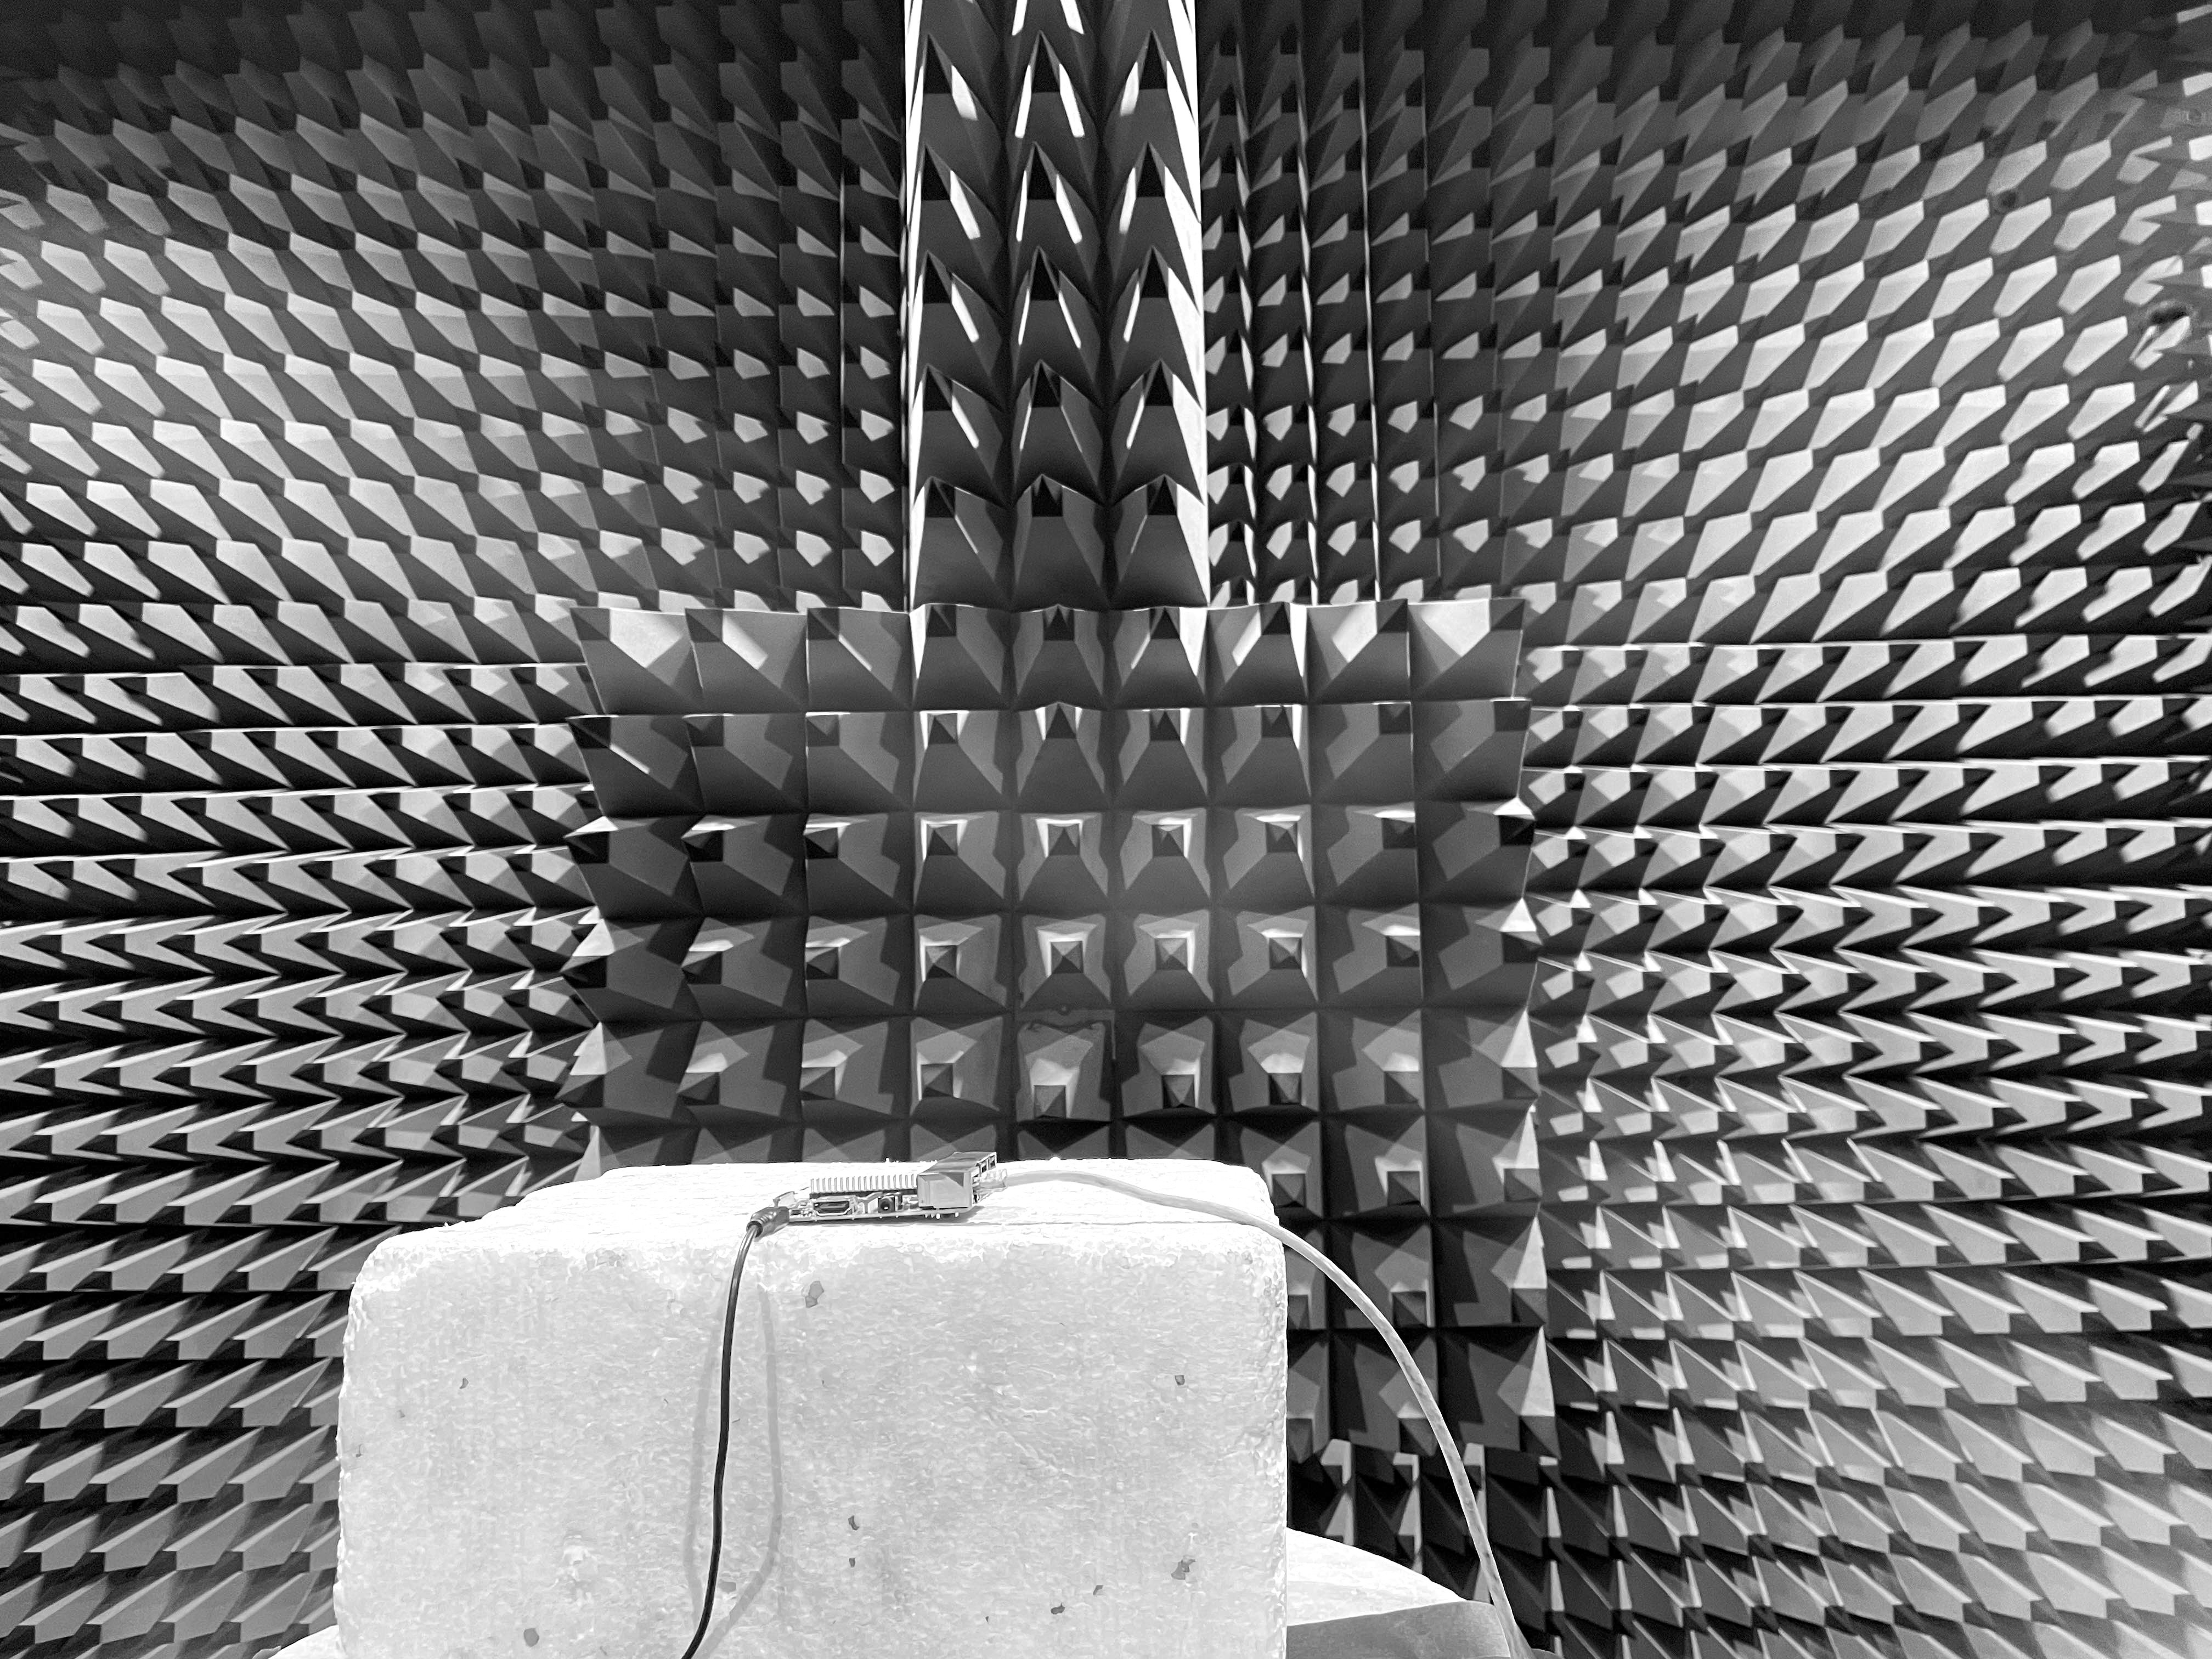
\includegraphics[width=0.8\textwidth]{fig/ch15/rasp_komora.jpg} % bez rozszerzenia
    \caption{Urządzenie Raspberry Pi 3 umieszczone w komorze kontroli szumu.}
    \label{fig:rasp_komora}
\end{figure}

\subsection{Konfiguracja urządzeń transmisyjnych}
Urządzenia transmisyjne to Raspberry Pi 3 z zainstalowanym na wymiennym nośniku pamięci systemem operacyjnym Raspberry Pi OS (Legacy, 32-bit). Dla każdego z pięciu urządzeń użyto tej samej karty micro-SD, co zagwarantowało urządzeniom te same ustawienia systemowe. Do skonfigurowania systemu jako punktu dostępu sieci wykorzystano otwarto-źródłowy sterownik \textit{hostapd}\footnote{~\url{https://manpages.debian.org/testing/hostapd/hostapd.8.en.html}}. Za kontrolę emisji wszystkich modułów radiowych (Wi-Fi, Bluetooth) odpowiadało również otwarto-źródłowe oprogramowanie \textit{rfkill}\footnote{~\url{https://linux.die.net/man/1/rfkill}}, którego użycie przedstawia listing ~\ref{listing:rfkill}.

Z ustawień przedstawionych na listingu ~\ref{listing:hostapd} szczególnie istotne dla przebiegu pomiarów były parametry, takie jak:
\begin{itemize}
    \item Nazwa sieci zdefiniowana jako "fingerprint".
    \item Częstotliwość nośna sygnału, zgodnie ze standardem \textit{channel=9}, definiuje środkową częstotliwość fali na 2452 MHz.
    \item Standard IEEE 802.11n zdefiniowany jako \textit{hw\_mode=n}.
    \item Okres rozgłaszania sygnału SSID jako \textit{beacon\_int=15}.
\end{itemize}
%\vspace{-4 mm}
\begin{listing}
\begin{minted}{shell}  
piotr@raspberrypi:~ $ cat /etc/hostapd/hostapd.conf
country_code=PL
interface=wlan0
ssid=fingerprint
channel=9
auth_algs=1
hw_mode=n
wpa=2
wpa_passphrase=korycki123
wpa_key_mgmt=WPA-PSK
wpa_pairwise=TKIP CCMP
rsn_pairwise=CCMP
beacon_int=15
\end{minted}
\caption{Plik konfiguracyjny routera hostapd} \label{listing:hostapd}
\end{listing}

\begin{listing}
\begin{minted}{shell}  
piotr@raspberrypi:~ $ rfkill list
0: phy0: Wireless LAN
        Soft blocked: no
        Hard blocked: no
1: hci0: Bluetooth
        Soft blocked: yes
        Hard blocked: no
\end{minted}
\caption{Odłączenie sygnału Bluetooth za pomocą rfkill} \label{listing:rfkill}
\end{listing}
%\vspace{-1 cm}
\subsection{Analizator widma Rohde \& Schwarz FSW-43}
Do zebrania sygnału referencyjnego, który informował o tym, czy sygnał jest nadawany prawidłowo, posłużyła aparatura pomiarowa, w którą była wyposażona komora EMC. Na rysunku ~\ref{fig:beacon_freq} została przedstawiona fala nośna o zdefiniowanej przez standard szerokości pasma 20 MHz, na której odbywa się transmisja sygnału SSID.
\begin{figure}[ht]
    \centering
    \includegraphics[width=0.7\textwidth]{fig/ch15/beacon.png} % bez rozszerzenia
    \caption{Zarejestrowany analizatorem widmowym sygnał w dziedzinie częstotliwości}
    \label{fig:beacon_freq}
\end{figure}
\subsection{Oscyloskop Tektronix MSO64B}
Dokładny przebieg amplitudy sygnału w czasie został zmierzony za pomocą oscyloskopu. Z uwagi na brak obsługi protokołu synchronizacji DSSS (Direct Sequence Spread Spectrum), w którym pracują urządzenia Wi-Fi 4, niemożliwym było zebranie prawidłowo zsynchronizowanego sygnału z częstotliwością próbkowania równą środkowej częstotliwości pasma. Przykład takiego błędu przedstawia wykres ~\ref{fig:sample_fault}.


\begin{figure}[ht]
    \centering
    \includegraphics[width=0.7\textwidth]{fig/ch15/sample_f_corr.png} % bez rozszerzenia
    \caption{Rozbieżność między transmitowanym oraz odbieranym sygnałem cyfrowym}
    \label{fig:sample_fault}
\end{figure}

W celu prawidłowej rekonstrukcji sygnału należy spełnić warunek twierdzenia Nyquista-Shannona, który mówi, że próbkowanie musi odbywać się z częstotliwością co najmniej dwukrotnie większą od szerokości pasma sygnału, a nie jego maksymalnej częstotliwości. Dla sygnału Wi-Fi o szerokości pasma $BW=20$ MHz wystarczy zatem częstotliwość próbkowania \( 40 \, \text{MHz} \), pod warunkiem sprowadzenia sygnału do pasma podstawowego. W praktyce parametry oscyloskopu pozwoliły na maksymalną częstotliwość próbkowania równą 25 GHz, co umożliwia poprawne próbkowanie sygnału o szerokości pasma 12,5 GHz. Oznacza to, że na każdy okres sygnału o częstotliwości 2462 MHz przypada od 9 do 10 próbek. Wysoka częstotliwość próbkowania umożliwia dokładną rejestrację sygnału oraz analizy zniekształceń, co demonstruje wykres ~\ref{fig:recon}.


\begin{figure}[ht]
    \centering
    \includegraphics[width=0.7\textwidth]{fig/ch15/rekonstrukcja.png} % bez rozszerzenia
    \caption{Rekonstrukcja sygnału dla stosunku próbkowania do transmisji 10:1}
    \label{fig:recon}
\end{figure}

Zgodnie z wyżej wymienionymi założeniami, na oscyloskopie zarejestrowano w formacie \textit{.mat} po 100 milionów próbek rzeczywistego sygnału Beacon dla wszystkich badanych płytek Raspberry Pi 3. Przykładowe prezentacje amplitudy w czasie dla płytki A zostały przedstawione na rysunkach ~\ref{fig:A_rela} i ~\ref{fig:A_rela50}. Należy jednak zwrócić uwagę na to, że zgodnie z wykresem ~\ref{fig:A_rela} oscyloskop jako sygnał referencyjny na początku oraz na końcu pomiaru zebrał również próbki szumu termicznego pomiędzy transmisjami, co można wywnioskować po tym, że zgodnie z konfiguracją routera ~\ref{listing:hostapd} oraz równaniem ~\ref{eq:timeVal}, okres przerwy między ramkami Beacon  wynosi 15,64 ms, a czas trwania całego zmierzonego sygnału to tylko 4 ms. Po odpowiednim przetworzeniu to właśnie te dane posłużyły do dalszej analizy opisanej w~pozostałej części pracy.

\begin{equation}
t = \frac{n}{f_s} = \frac{10^8}{2.5 \times 10^{10}} = 0.004 \, \text{s}
\label{eq:timeVal}
\end{equation}

\noindent gdzie:
\begin{itemize}
    \item $t$ - czas trwania sygnału,
    \item $f_s$ - częstotliwość próbkowania,
    \item $n$ - liczba próbek sygnału.
\end{itemize}


\begin{figure}[ht]
    \centering
    \includegraphics[width=0.7\textwidth]{fig/ch15/A_real.png} % bez rozszerzenia
    \caption{Zarejestrowany oscyloskopem sygnał dla płytki o etykiecie A (100 milionów próbek)}
    \label{fig:A_rela}
\end{figure}

\begin{figure}[ht]
    \centering
    \includegraphics[width=0.7\textwidth]{fig/ch15/A_real_50.png} % bez rozszerzenia
    \caption{Zarejestrowany oscyloskopem sygnał dla płytki o etykiecie A (50 tysięcy próbek)}
    \label{fig:A_rela50}
\end{figure}

\subsection{Wstępne przetwarzanie danych}
W celu dalszej analizy surowe dane pozyskane z oscyloskopu są przetwarzane aby usunąć z nagrania sygnału nadmiarowe dane oraz aby przetransformować sygnał rzeczywisty na reprezentację IQ.
\subsubsection{Format danych wejściowych}
Zgodnie z ustaleniami z poprzedniego rozdziału do dalszej części projektu posłużyły próbki sygnału oraz czasu zarejestrowane przez oscyloskop Tektronix MSO64B zapisane w formacie \textit{.mat}. Na przykładowym nagraniu sygnału w dziedzinie czasu przedstawionym na wykresie ~\ref{fig:A_rela} można zaobserwować, że duża część zebranych próbek to referencyjny szum termiczny, który na etapie analizy różnicy w transmisjach poszczególnych urządzeń Raspberry Pi 3 nie jest uwzględniany. Ponadto, analiza ma dotyczyć sygnału w~formacie IQ. Ponieważ wyniki pomiarów zostały zapisane w formacie \textit{.mat} który zawiera sygnał rzeczywisty dlatego konieczna jest transformacja do IQ w oparciu o dostępne metadane sygnału (częstotliwość środka pasma).
\subsubsection{Algorytmy wycinania szumu termicznego}
Celem algorytmów zaproponowanych w tej sekcji jest odseparowanie sygnału od stanowiących początek i koniec nagrania próbek szumu termicznego. Jak widać na wykresie ~\ref{fig:sig_begin}, w nagraniu sygnału również są zarejestrowane próbki o niskiej amplitudzie, w związku z czym niemożliwym było podzielenie próbek według kryterium wysokości amplitudy. W celu rozwiązania tego problemu pierwszym krokiem algorytmu jest podzielenie nagrania na równe odcinki o ustalonej długości i wyliczenie na ich podstawie lokalnych maksimów.

\begin{figure}[ht]
    \centering
    \includegraphics[width=0.8\textwidth]{fig/ch15/poczatek.png} % bez rozszerzenia
    \caption{Przejście szumu w sygnał.}
    \label{fig:sig_begin}
\end{figure}
\paragraph{\textit{Algorytm DecMax}}
Przedstawiony na listingu ~\ref{alg:dec_max} algorytm DecMax realizuje decymację sygnału na lokalne maksima przedziałów o zadanej długości, na podstawie których można analizować dane pod kątem trendu, a nie zawierających próbki szumu i sygnału pojedynczych wartości amplitudy. Ze względu na to, że sygnał oscyluje wokół ujemnych i dodatnich wartości napięcia, konieczne jest wyliczanie maksimów po wartości bezwzględnej amplitudy.
% \begin{algorithm}
% \caption{Decymacja sygnału z maksymalną wartością w przedziale}\label{alg:dec_max}
% \begin{algorithmic}[1]
% \Function{DecMax}{\textit{signal}, $n$}
%     \State \textit{m} $\gets \lfloor\frac{\textit{length(signal)} - n}{n}\rfloor + 1$\;
%     \State \textit{decimated} $\gets [1, \dots, m]$\;
%     \For{$i = 1$ \textbf{to} \textit{length(signal)} $- n$ \textbf{step} $n$}
%         \State \textit{window\_max} $\gets \max\left(\left| \textit{signal}[i : i+n] \right|\right)$\;
%         \State $\textit{decimated}[i] \gets \textit{window\_max}$\;
%     \EndFor
%     \State \Return \textit{decimated}
% \EndFunction
% \end{algorithmic}
% \end{algorithm}

\begin{algorithm}[H]
\DontPrintSemicolon
\LinesNumbered
\SetKwInOut{Input}{Input}
\SetKwInOut{Output}{Output}

\Input{signal, $n$}
\Output{decimated signal}

\BlankLine
$m \gets \lfloor (\text{length(signal)} - n)/n \rfloor + 1$\;
decimated $\gets$ array of length $m$\;

\For{$k \gets 0$ \textbf{to} $m-1$}{
    $i \gets k \cdot n + 1$\;
    window\_max $\gets \max(|\text{signal}[i : i+n]|)$\;
    decimated[$k+1$] $\gets$ window\_max\;
}

\Return decimated\;
\caption{Decymacja sygnału z maksymalną wartością w przedziale}
\label{alg:dec_max}
\end{algorithm}


Przykład sygnału po decymacji przedstawiony jest na wykresie ~\ref{fig:max}.
\begin{figure}[ht]
    \centering
    \includegraphics[width=0.7\textwidth]{fig/ch15/maksima.png} % bez rozszerzenia
    \caption{Przykład lokalnych maksimów sygnału dla przedziałów o~długości 10000 próbek.}
    \label{fig:max}
\end{figure}

\paragraph{\textit{Algorytm DegMax}}
Po otrzymaniu maksimów sygnału po decymacji możliwe jest ustalenie metody detekcji zmiany trendu. Jak można wywnioskować z wykresu ~\ref{fig:straights} punkty charakterystyczne dla początku (ale również końca) sygnału odznaczają się dużą różnicą amplitudy w stosunku do próbek szumu. Jeśli każde kolejne dwa punkty zostaną połączone odcinkiem prostym (kolor czerwony), można zauważyć, że kąt $\alpha$, jaki odcinek tworzy z prostą o równaniu $y=0$, odwzorowuje wspomniane wahania amplitudy i~jest możliwy do obliczenia zgodnie ze wzorem ~\ref{eq:degree}.

\begin{equation}
\alpha = \arctan(\tan(\alpha)) = \arctan(\frac{|a_1 - a_2|}{d}),
\label{eq:degree}
\end{equation}
gdzie
\begin{itemize}
    \item $a_1$, $a_2$-amplitudy dwóch kolejnych próbek
    \item $d$-ustalona odległość między próbkami, może wynosić 1
\end{itemize}

\begin{figure}[ht]
    \centering
    \includegraphics[width=0.75\textwidth]{fig/ch15/maks_przejscie.png} % bez rozszerzenia
    \caption{Przykład lokalnych maksimów sygnału dla przedziałów o~długości 10000 próbek z naniesionymi prostymi.}
    \label{fig:straights}
\end{figure}

Na bazie powyższych wniosków celem algorytmu jest obliczenie kątów między odcinkami łączącymi kolejne próbki, a prostą o równaniu $y=0$. Pseudokod algorytmu przedstawia listing ~\ref{alg:fill_deg}. Przykładowe wyniki algorytmów DecMax i~DegMax zostały umieszczone na wykresie ~\ref{fig:trim_logs}. Jak można zaobserwować na przecięciu sygnału oraz szumu, wartości kątów są największe, co stanowi kryterium cięcia.

% \begin{algorithm}
% \caption{Obliczanie kątów między sąsiednimi próbkami sygnału}\label{alg:fill_deg}
% \begin{algorithmic}[1]
% \Function{DegMax}{\textit{signal}, $d$}
%     \State \textit{n} $\gets \textit{length(signal)} - 2$
%     \State \textit{degrees} $\gets [1, \dots, n]$
%     \For{$i = 1$ \textbf{to} \textit{length(signal)} $- 2$}
%         \State \textit{diff} $\gets \left|\textit{signal}[i] - \textit{signal}[i+1]\right|$
%         \State \textit{angle} $\gets \arctan\left(\frac{\textit{diff}}{d}\right)$
%         \State $\textit{degrees}[i] \gets \textit{angle}$
%     \EndFor
%     \State \Return \textit{degrees}
% \EndFunction
% \end{algorithmic}
% \end{algorithm}

\begin{algorithm}[H]
\DontPrintSemicolon
\LinesNumbered
\SetKwInOut{Input}{Input}
\SetKwInOut{Output}{Output}
\Input{signal, $d$}
\Output{degrees between consecutive signal samples}
\BlankLine
$n \gets \text{length(signal)} - 2$\;
degrees $\gets$ array of length $n$\;
\For{$i \gets 1$ \KwTo length(signal) $- 2$}{
    diff $\gets |\text{signal}[i] - \text{signal}[i+1]|$\;
    angle $\gets \arctan(diff / d)$\;
    degrees[$i$] $\gets$ angle\;
}
\Return degrees\;
\caption{Obliczanie kątów między sąsiednimi próbkami sygnału}
\label{alg:fill_deg}
\end{algorithm}



\begin{figure}[ht]
    \centering
    \includegraphics[width=0.8\textwidth]{fig/ch15/probka_E_25GS_logs.png} % bez rozszerzenia
    \caption{Wykresy lokalnych maksimów oraz kątów nachylenia prostych dla sygnału płytki E i długości przedziałów równej 10000.}
    \label{fig:trim_logs}
\end{figure}

\paragraph{\textit{Algorytm TriMax}}
Algorytm przycinania sygnału (TriMax) działa z wykorzystaniem informacji dostarczonych przez powyższe rozwiązania. TriMax korzysta również z funkcji $twomax(wektor)$, która stanowi prostą modyfikację algorytmu wyszukiwania elementu maksymalnego, zwracającą indeksy dwóch największych elementów w wektorze w czasie liniowym. Metoda ta polega na wyznaczeniu krańców sygnału na podstawie dwóch maksymalnych wartości kątów i przycięciu danych o amplitudzie i czasie w tak wyznaczonych granicach. Listing ~\ref{listing:trimax} przedstawia zastosowaną w projekcie implementację algorytmu w języku Julia. Złożoność algorytmu $T(n)$, liczona jako suma złożoności wywołanych pojedynczo funkcji, wynosi $O(n)$, ponieważ każda z nich ma złożoność również $O(n)$.
\begin{listing}[H]
\begin{minted}{julia}
function TriMax(signal, time; n=10000)
    decimated_max = DecMax(signal, n=n)
    degrees = DegMax(decimated_max)
    i, j = TwoMax(angles)
    i *= n
    j *= n
    if (i < j)
        return signal[i:j], time[i:j]
    else
        return signal[j:i], time[j:i]
    end
end
\end{minted}
\caption{Implementacja algorytmu TriMax w języku Julia.} \label{listing:trimax}
\end{listing}

% \subsubsection{Demodulacja sygnału}
% W celu doprowadzenia sygnału do formy, w jakiej nadajnik prowadził transmisję, należało dodatkowo zdemodulować dane w oparciu o schemat modulacji QAM. Schemat modulacji przedstawiony na diagramie ~\ref{fig:qam_mod} demonstruje, że wyemitowana fala to w rzeczywistości suma dwóch sygnałów przesuniętych w fazie o $90^{\circ}$. W celu odwrócenia procesu modulacji wystarczyło więc przemnożyć zarejestrowany sygnał przez fale o częstotliwości $f_c=2452$ MHz określone równaniami ~\ref{eq:I_carrier} oraz ~\ref{eq:Q_carrier}. Listing ~\ref{listing:demod} przedstawia zastosowaną w programie implementację demodulacji kwadraturowo-amplitudowej.
% \begin{equation}
% I_{carrier}= \cos(2\pi f_c t) \label{eq:I_carrier}
% \end{equation}
% \begin{equation}
% Q_{carrier} = \sin(2\pi f_c t) \label{eq:Q_carrier}
% \end{equation}


% %Listing ~\ref{listing:demod} przedstawia zastosowaną w programie implementację demodulacji kwadraturowo-amplitudowej.

% \begin{figure}[ht]
%     \centering
%     \includegraphics[width=0.8\textwidth]{fig/ch15/generation-of-QAM-signal.png} % bez rozszerzenia
%     \caption{Schemat modulacji QAM na podstawie \cite{qam_website}.}
%     \label{fig:qam_mod}
% \end{figure}

% \begin{listing}
% \begin{minted}{julia}
% function demodulate(signal, t; carrier_freq=2.452e9)
%     I_carrier = cos.(2 * pi * carrier_freq .* t)
%     Q_carrier = sin.(2 * pi * carrier_freq .* t)
%     return signal .* I_carrier, signal .* Q_carrier
% end
% \end{minted}
% \caption{Implementacja demodulacji QAM w języku Julia.} \label{listing:demod}
% \end{listing}
\subsubsection{Aplikacja Trimmer}
Program służący do wstępnej obróbki danych pomiarowych przed etapem dalszej analizy został napisany z wykorzystaniem powyższych algorytmów. Aplikacja została zaimplementowana w języku Julia ze względu oraz obsługę plików w~formacie \textit{.mat}. Przy wywołaniu z linii komend program przyjmuje następujące argumenty:
\begin{itemize}
    \item \texttt{---upscale} włącza konwersję jednostki amplitudy na mV.
    \item \texttt{---raw} pozwala na zapisanie przyciętego sygnału w postaci rzeczywistej bez transformacji na format IQ.
    % \item Flaga \texttt{---iq} pozwalająca na zapisanie przyciętego sygnału w postaci zdemodulowanej.
    \item \texttt{---input} po którym należy wpisać ścieżkę pliku wejściowego w formacie \textit{.mat}.
    \item \texttt{---frequency} określająca częstotliwość fali nośnej w MHz potrzebną do demodulacji sygnału.
    \item \texttt{---verbose} umożliwia zapisanie wykresów parametrów, a także odcinków początku i końca sygnału dla zwiększenia ilości informacji o~procesie przetwarzania danych.
    \item \texttt{title} pozwala określić tytuł wykresów generowanych w trybie \texttt{verbose}.
\end{itemize}
Po zakończeniu działania program Trimmer zapisuje przycięte dane ponownie w formacie \textit{.mat}. Efekty działania aplikacji zostały zaprezentowane na wykresie ~\ref{fig:trim_begin}.%, ~\ref{fig:trim_demod} i ~\ref{fig:trim_const}.
\begin{figure}[ht]
    \centering
    \includegraphics[width=0.8\textwidth]{fig/ch15/probka_E_25GS_begin.png} % bez rozszerzenia
    \caption{Wykres początku przyciętego sygnału dla płytki E.}
    \label{fig:trim_begin}
\end{figure}

% \begin{figure}[ht]
%     \centering
%     \includegraphics[width=0.8\textwidth]{fig/ch15/timedomainiq.png} % bez rozszerzenia
%     \caption{Wykres zdemodulowanego sygnału dla płytki E.}
%     \label{fig:trim_demod}
% \end{figure}

% \begin{figure}[ht]
%     \centering
%     \includegraphics[width=0.8\textwidth]{fig/ch15/constellationiq.png} % bez rozszerzenia
%     \caption{Wykres konstelacji sygnału po demodulacji dla płytki E.}
%     \label{fig:trim_const}
% \end{figure}


\section{Analiza i klasyfikacja danych}
W tej sekcji przedstawione są metody analizy wstępnie przetworzonych próbek. Celem analizy jest zbadanie możliwości klasyfikacji urządzeń dzięki unikalnym niedoskonałościom urządzeń transmisyjnych, a w szczególności niedoskonałościach balansu amplitudy.
% \subsection{Przesunięcie sygnału w fazie}
% W celu zbadania przebiegu fazy sygnału w czasie oraz ewentualnych różnic w otrzymanych wynikach pomiędzy testowanymi urządzeniami należało zaimplementować algorytm zliczający narastające opóźnienie fazy. Wejściem programu były zdemodulowane dane otrzymane za pomocą algorytmu TriMax, a efektem pracy algorytmu były dane przedstawiające zmianę fazy na przestrzeni zarejestrowanego sygnału.
% \paragraph{Analiza centroidów}
% Z uwagi na to, że posługujemy się rekonstrukcją, a nie zsynchronizowanymi próbkami wyemitowanego sygnału, koniecznym było wyznaczenie takiej wielkości próbki danych, jaka będzie reprezentatywna dla wszystkich rejestrowanych wartości centroidu. Jak widać na wykresach ~\ref{fig:iq10k}, przykładowy przedział zawierający 10 000 symboli IQ jest niewystarczający, więc w dalszej części badań pojedyncza próbka konstelacji miała długość 100 000 symboli.

% \begin{figure}[ht] 
% 	\centering
% 	\begin{minipage}[b]{0.45\textwidth}
% 		\centering\includegraphics[width=0.9\textwidth]{fig/ch15/c10k.png} % left figure
% 	\end{minipage}
% 	\begin{minipage}[b]{0.45\textwidth}
% 		\centering
% 		\includegraphics[width=0.9\textwidth]{fig/ch15/c100k.png} % right figure
% 	\end{minipage}
%     \caption{Porównanie wykresów konstelacji zdemodulowanego sygnału dla płytki E}\label{fig:iq10k}
% \end{figure}

% Jeśli nałożymy na siebie wykresy dwóch kolejnych odcinków (wykres ~\ref{fig:c200k}), możemy zaobserwować wyraźny obrót następujących po sobie centroidów wokół punktu $(0,0)$. Jest to nic innego jak rotacja liczb zespolonych składających się na przedstawione centroidy o dany kąt $\phi$ równy skumulowanemu przesunięciu w fazie sygnału. Dzięki analizie rotacji centroidów możliwe było oszacowanie charakterystyki badanego nadajnika, do czego posłużył Algorytm Detekcji Oszacowanej Fazy.
% \begin{figure}[ht]
%     \centering
%     \includegraphics[width=0.8\textwidth]{fig/ch15/c200k.png} % bez rozszerzenia
%     \caption{Wykres konstelacji dwóch odcinków zdemodulowanego sygnału dla płytki E.}
%     \label{fig:c200k}
% \end{figure}

% \subsubsection{Algorytm detekcji oszacowanej fazy}
% ADOF, przedstawiony w pseudokodzie ~\ref{alg:ADOF}, dzieląc sygnał na odcinki długości $k$, w pierwszym kroku klasyfikuje centroidy za pomocą algorytmu k-średnich. Ze względu na wysoką precyzję wykonanych pomiarów oraz fakt, że zebrane próbki zawierają również szum termiczny, na każdym wykresie konstelacji nastąpiła duża koncentracja danych wokół punktu $(0,0)$, co doprowadziło do sytuacji, w której kMeans nie mógł poprawnie sklasyfikować dwóch centroidów. Przykład pochłaniania jednego centroidu przez drugi wokół obszaru niskich amplitud przedstawia wykres ~\ref{fig:pochlanianie}. W celu uniknięcia błędnej klasyfikacji, do wejścia algorytmu k-średnich dodany został trzeci centroid niskich amplitud rozpoznawany po tym, że jego odległość w metryce euklidesowej od punktu $(0,0)$ jest najmniejsza. Centroidy $\alpha$ i $\beta$ są przypisywane w dowolnej kolejności.

% W dalszej części algorytm, iterując po kolejnych przedziałach długości $k$, ponownie wylicza środki centroidów, a następnie klasyfikuje je w oparciu o odległość euklidesową od środka centroidu poprzedniego przedziału. Faza tak sklasyfikowanych punktów obliczana jest ze współrzędnych poprzez rozszerzenie funkcji $\arctan()$, która dla uniknięcia wartości ujemnych zwraca kąt z przedziału $[0, 2\pi]$. Każde wywołanie funkcji $\textit{collectCenters(centroids\_map, center\_alpha, center\_beta, mid\_point, c)}$ uzupełnia wektory przypisane w strukturze \textit{centroids\_map} do centroidów $\alpha$, $\beta$ i \textit{S} o podane punkty na pozycji \textit{c}.


% Implementację struktury centroids\_map w języku Python, która służy do przechowywania danych o współrzędnych i fazie środków centroidów, przedstawia listing ~\ref{listing:map}.

% \begin{listing}
% \begin{minted}{python}
% import numpy as np
% iter = n//k
% one_centroid_map = {
%         "I": np.zeros(iter),
%         "Q": np.zeros(iter),
%         "phase": np.zeros(iter)
%     }
% centroids_map = {
%     "A": one_centroid_map,
%     "S": one_centroid_map,
%     "B": one_centroid_map
% }
% \end{minted}
% \caption{Implementacja struktury danych odpowiadającej za przechowywanie informacji o centroidach.} \label{listing:map}
% \end{listing}


% \begin{figure}[ht] 
% 	\centering
% 	\begin{minipage}[b]{0.45\textwidth}
% 		\centering\includegraphics[width=1\textwidth]{fig/ch15/clusters22_E.png} % left figure
% 	\end{minipage}
% 	\begin{minipage}[b]{0.45\textwidth}
% 		\centering
% 		\includegraphics[width=1\textwidth]{fig/ch15/clusters2_E.png} % right figure
% 	\end{minipage}
%     \caption{Porównanie klasyfikacji centroidów zdemodulowanego sygnału dla płytki E}\label{fig:pochlanianie}
% \end{figure}

% \begin{algorithm}
% \caption{Algorytm ADOF do analizy sygnałów I i Q}\label{alg:ADOF}
% \begin{algorithmic}[1]
% \Function{ADOF}{\textit{I}, \textit{Q}, $n$, $k \gets 100000$}
%     \State $c \gets 1$
%     %\State \textit{iter} $\gets \lfloor \frac{n}{k} \rfloor$
%     \State \textit{centroids\_map} $\gets$ pusty słownik
%     \State \textit{centers} $\gets$ \textit{kMeans}(\textit{I}[1:$k$], \textit{Q}[1:$k$], 3)
%     \State \textit{distances} $\gets$ \textit{Euclidean}((0, 0), \textit{centers})
%     \State $i_{\text{mid}} \gets \textit{argMin}(\textit{distances})$
%     \State \textit{mid\_point} $\gets$ \textit{centers}[$i_{\text{mid}}$]
%     \State \textit{erase}(\textit{centers}, \textit{mid\_point})
%     \State \textit{collectCenters}(\textit{centroids\_map}, \textit{centers}[1], \textit{centers}[2], \textit{mid\_point}, \textit{c})
%     \State $c \gets c + 1$

%     \For{$i = k$ \textbf{to} $n - k$ \textbf{step} $k$}
%         \State \textit{centers} $\gets$ \textit{kMeans}(\textit{I}[$i:i+k$], \textit{Q}[$i:i+k$], 3)
%         \State \textit{distances} $\gets$ \textit{Euclidean}((0, 0), \textit{centers})
%         \State $i_{\text{mid}} \gets \textit{argMin}(\textit{distances})$
%         \State \textit{mid\_point} $\gets$ \textit{centers}[$i_{\text{mid}}$]
%         \State \textit{erase}(\textit{centers}, \textit{mid\_point})
%         \State \textit{distances\_alpha} $\gets$ \textit{Euclidean}(\textit{getAlpha}(\textit{centroid\_map}), \textit{centers})
%         \State \textit{distances\_beta} $\gets$ \textit{Euclidean}(\textit{getBeta}(\textit{centroid\_map}), \textit{centers})
%         \State \textit{center\_alpha} $\gets$ \textit{centers}[\textit{argMin}(\textit{distances\_alpha})]
%         \State \textit{center\_beta} $\gets$ \textit{centers}[\textit{argMin}(\textit{distances\_beta})]
%         \State \textit{collectCenters}(\textit{centroids\_map}, \textit{center\_alpha}, \textit{center\_beta, \textit{mid\_point}, \textit{c}})
%         \State $c \gets c + 1$
%     \EndFor
%     \State \Return \textit{centroids\_map}
% \EndFunction
% \end{algorithmic}
% \end{algorithm}

% \subsubsection{Analiza złożności algorytmu ADOF}
% Algorytm wykonując pętlę o długości $\lfloor \frac{n}{k} \rfloor$ w każdym kroku:
% \begin{enumerate}
%     \item Wywołuje algorytm k-średnich dla:
%     \begin{itemize}
%         \item Dwóch wymiarów danych $d$.
%         \item Trzech klastrów $a$.
%         \item Domyślnej liczby iteracji konwergencji $i=20$.
%         \item Rozmiaru wektorów $I$ i $Q$ równego k.
%     \end{itemize}
%     \item W stałym czasie klasyfikuje środki centroidów.
%     \item W stałym czasie uzupełnia strukturę centroid\_map o wyliczone dane.
% \end{enumerate}
% Zgodnie ze specyfikacją algorytmu k-średnich w bibliotece SciPy \cite{scipy_kmeans_reference}, funkcja ta jest określona złożonością $O(a\cdot d\cdot i \cdot k)$, stąd ADOF ma złożoność $\theta(\lfloor \frac{n}{k} \rfloor)\cdot O(a\cdot d\cdot i \cdot k) = O(\lfloor \frac{n}{k} \rfloor)\cdot O(3\cdot 2\cdot i \cdot k) = O(n\cdot i)$.

% \subsubsection{Interpretacja wyników}
% Algorytm poprawnie zarejestrował przebieg fazy sygnału dla wszystkich badanych płytek. Wykresy ~\ref{fig:mids} przedstawiają położenie wszystkich zarejestrowanych środków ciężkości. Dla lepszej prezentacji wyniku współrzędne centroidu $\alpha$ zostały przesunięte o wektor $(5,5)$.

% Na wykresie ~\ref{fig:phase} została przedstawiona zakumulowana faza sygnału w czasie. Wykres ~\ref{fig:vectors} ilustruje fragment rotacji centroidu.

% \begin{figure}[ht] 
% 	\centering
% 	\begin{minipage}[b]{0.45\textwidth}
% 		\centering\includegraphics[width=1\textwidth]{fig/ch15/centers_shifted_D.png} % left figure
% 	\end{minipage}
% 	\begin{minipage}[b]{0.45\textwidth}
% 		\centering
% 		\includegraphics[width=1\textwidth]{fig/ch15/centers_shifted_E.png} % right figure
% 	\end{minipage}
%     \caption{Przebieg położenia środków centroidów.}\label{fig:mids}
% \end{figure}

% \begin{figure}[ht] 
% 	\centering
% 	\begin{minipage}[b]{0.45\textwidth}
% 		\centering\includegraphics[width=1\textwidth]{fig/ch15/phase_sum_D.png} % left figure
% 	\end{minipage}
% 	\begin{minipage}[b]{0.45\textwidth}
% 		\centering
% 		\includegraphics[width=1\textwidth]{fig/ch15/phase_sum_E.png} % right figure
% 	\end{minipage}
%     \caption{Suma krocząca fazy centroidów}\label{fig:phase}
% \end{figure}

% \begin{figure}[ht]
%     \centering
%     \includegraphics[width=0.8\textwidth]{fig/ch15/centers_shifted_arrow_E.png} % bez rozszerzenia
%     \caption{Wykres przebiegu położenia środka centroidu z naniesionym kierunkiem rotacji dla płytki E.}
%     \label{fig:vectors}
% \end{figure}
% Wyniki działania algorytmu dla wszystkich urządzeń z fazą mierzoną w radianach zostały zaprezentowane w tabeli ~\ref{table:phase}.
%     \begin{table}[ht]
% \centering
% \caption{Wyniki analizy przebiegu fazy liczonej w radianach.}
% \label{table:phase}
% \begin{tabular}{|c|c|c|c|}
% \hline

% 			\textbf{Płytka} & \textbf{Faza centroidu $\alpha$} & \textbf{Faza centroidu $\beta$} & \textbf{Liczba przedziałów}\\
% \hline
% 			A & 1230.11 & 1221.71 & 398 \\
%             \hline
% 			B & 1311.69 & 1301.20 & 398 \\
%             \hline
% 			C & 1161.54 & 1086.44 & 398 \\
%             \hline
%             D & 1224.98 & 1216.63 & 398 \\
%             \hline
%             E & 1269.37 & 1261.05 & 398 \\
%             \hline

% 		\end{tabular}

        
% 	\end{table}

\subsection{Niedoskonałości w amplitudzie}
W tej części opisane jest przystosowanie modelu neuronowej sieci konwolucyjnej, której głównym zadaniem jest rozpoznawanie fotografii, do klasyfikacji sygnału urządzeń po niedoskonałościach w wartości amplitudy. Motywacją do zastosowania tego modelu są obiecujące wyniki klasyfikacji sygnału opisane w pracy \cite{sankhe2019oracle}. W~tradycyjnym zastosowaniu modele neuronowych sieci konwolucyjnych jako dane wejściowe przyjmują wektorowe reprezentacje fotografii jako 3 kanały odpowiadające za wartości pikseli w domenie koloru (w reprezentacji r,g,b). 
% Pomysłem na modyfikację takiego modelu było wprowadzenie reprezentacji wektorowej jednego diagramu konstelacji IQ jako dwa kanały I i Q o długości 100000 próbek. Do implementacji modelu zastosowano bibliotekę PyTorch \cite{pytorch}.
\subsubsection{Klasa IQDataset}
IQDataset, przedstawiony na Listingu ~\ref{listing:dataset}, to klasa dziedzicząca po interfejsie Dataset w bibliotece PyTorch. Danymi wejściowymi klasy jest słownik porządkujący pary wektorów I i Q według etykiet urządzeń $\{A, B, C, D, E\}$. Nadpisana metoda \textit{\_\_get\_\_item()} odpowiada za konwersję sygnału do tensora, a także przepisanie etykiet urządzeń na akceptowane przez sieć neuronową liczby $\{0,1,2,3,4\}$.
\begin{listing}[H]
\begin{minted}[breaklines, breakanywhere]{python}
import torch
from torch.utils.data import Dataset, DataLoader
class IQDataset(Dataset):
    def __init__(self, training_data):
        total_samples = sum(len(data['I']) for data in training_data.values())
        self.samples = [None] * total_samples
        current_idx = 0
        for device, data in training_data.items():
            I_data = data['I']
            Q_data = data['Q']
            for i in range(len(I_data)):
                self.samples[current_idx] = {
                    'device': device,
                    'I': I_data[i],
                    'Q': Q_data[i],
                }
                current_idx += 1
    def __len__(self):
        return len(self.samples)
    def __getitem__(self, idx):
        sample = self.samples[idx]
        return {
            'input': torch.tensor([sample['I'], sample['Q']], dtype=torch.float32),
            'label': torch.tensor(label_to_tens(sample['device'])),
        }
\end{minted}
\caption{Implementacja klasy IQDataset w języku Python.} \label{listing:dataset}
\end{listing}
\subsubsection{Model sieci neuronowej}
W projekcie użyto sieci IQCNN, podobnej do modelu klasyfikacji sygnału przedstawionego w pracy \cite{sankhe2019oracle}. Sieć została zaprojektowana z myślą o odwzorowaniu procesu uczenia głębokiego dla obrazów na przetwarzanie diagramów konstelacji sygnału. Model można podzielić na następujące warstwy:
\begin{enumerate}
    \item Warstwa wejściowa o rozmiarze $1\times N \times 2$, gdzie $N=100000$.
    \item Pierwsza warstwa konwolucyjna odpowiadająca za ekstrakcję lokalnych cech i implementację filtrów. Warstwa ta posiada 16 filtrów, każdy o rozmiarze 5. Wejście warstwy ma rozmiary $(batch\_size, 2, 100000)$, a wyjście $(batch\_size, 16, 100000)$.
    \item Pierwsza warstwa Max Pooling odpowiadająca za redukcję wymiarowości danych. Wyjściowa wielkość danych to $(batch\_size, 16, 50000)$.
    \item Druga warstwa konwolucyjna odpowiadająca za dalsze wyszukiwanie cech posiada 32 filtry, również o rozmiarze 5. Finalnie całkoiwty rozmiar wyjścia wynosi $(batch\_size, 32, 50000)$.
    \item Druga warstwa Max Pooling odpowiadająca za spłaszczenie danych przed dalszym przetwarzaniem. Rozmiar wyjścia to $(batch\_size, 32, 25000)$.
    \item Warstwa spłaszczająca Flatten odpowiadająca za spłaszczenie danych przed dalszym przetwarzaniem. Wyjściowe wymiary tensora to $(batch\_size, 32\cdot 25000)$.
    \item Pierwsza warstwa w pełni połączona Fully Connected odpowiadająca za połączenie wejściowych neuronów do tensora o wymiarach $(batch\_size,128)$.
    \item Druga warstwa w pełni połączona odpowiadająca za końcową klasyfikację danych.
\end{enumerate}
Poglądowy schemat architektury sieci został opracowany w środowisku AlexNet\footnote{~\url{https://alexlenail.me/NN-SVG/AlexNet.html}} i jest przedstawiony na diagramie ~\ref{fig:alexnet}.
\begin{figure}[ht]
    \centering
    \includegraphics[width=0.7\textwidth]{fig/ch15/cnn_subtitled.png} % bez rozszerzenia
    \caption{Schemat architektury modelu IQCNN z oznaczeniami warstw oraz rozmiarami filtrów.}
    \label{fig:alexnet}
\end{figure}

% Proces trenowania modelu składa się z dziesięciu iteracji, w których zastosowano parametr liczby próbek przetwarzanych równolegle $batch\_size=64$. Obliczenia zotsały przeprowadzone na procesorze Intel Core i7-1270P 2.20 GHz dla $5\times39\times10^{9}$ próbek IQ trwały 27 minut, a końcowa dokładność treningu wyniosła 96,97\%. W trakcie tego procesu IQCNN wykształcił w sobie łączny zestaw cech rozmiaru 102403541 parametrów.

Do ewaluacji modelu użytych zostało $5\times8\times10^{5}$ próbek IQ, będących zbiorem rozłącznym od sygnału użytego w trakcie uczenia sieci, choć zarejestrowanym w~tych samych warunkach otoczenia. W trakcie ewaluacji przeprowadzone zostało łącznie 40 testów dla wszystkich urządzeń transmisyjnych, w których model poprawnie poprawnie klasyfikował etykietę urządzenia 36 razy, co daje końcową dokładność 90\%.

\section{Wnioski i podsumowanie}

W pracy zaproponowano metodę akwizycji sygnałów WiFi poprzez przeprowadzenie pomiarów na oscyloskopie Tektronix MSO64B. Zaimplementowano autorskie oprogramowanie mające na celu obróbkę surowych danych z oscyloskopu i klasyfikację sygnału testowanych urządzeń. Spełnia to najważniejsze założenie projektu oraz tworzy podstawy dla dalszego rozwoju technologii identyfikacji urządzeń nadawczych przy użyciu uczenia maszynowego. Przedstawione w pracy algorytmy wstępnego przetwarzania sygnału radiowego w czasie liniowym oraz modele klasyfikacji urządzeń po niedoskonałościach w emitowanym sygnale wykazały bardzo obiecujące wyniki,  90\% skutecznych identyfikacji w warunkach testowych, co uzasadnia kontynuację prac.
%
Proponowane dalsze kierunki badań i~rozwoju projektu to:
\begin{enumerate}   
 %   \item Oprogramowanie na układzie FPGA radia RFSoC 4x2 protokołu synchronizacji sygnału OFDM w celu odejścia od rekonstrukcji sygnału cyfrowego i zwiększenia wydajności przeprowadzanych pomiarów. Taka funkcjonalność umożliwiłaby także rejestrację sygnału w moulacjach wyższego rzędu, a także przeprowadzanie pomiarów na znacznie większym wachlarzu urządzeń, w tym m.in. na telefonach komórkowych.
    \item Zwiększenie liczby badanych urządzeń w celu dalszego rozwoju i testowania modelu IQCNN.
    \item Modyfikacja architektury sieci IQCNN w celu uwzględnienia i identyfikacji urządzeń nieuwzględnionych podczas trenowania sieci.
    \item Testowanie sieci IQCNN w rzeczywistych warunkach propagacyjnych z~uwzględnieniem kanału komunikacyjnego.
    \item Użycie dedykowanej i mobilnej platformy do akwizycji i lokalnego przetwarzania sygnałów, np. platformy RFSoC 4x2 firmy RealDigital,  oraz stworzenie infrastruktury odbiorczej dla łącza o wysokiej przepustowości w celu zmniejszenia kosztów prowadzenia badań.
\end{enumerate}

\begin{thebibliography}{20}

\bibitem{rf_fingerprinting_sciencedirect}
  Jagannath, A., Jagannath, J., and Kumar, P. S. P. V.: RF Fingerprinting: New Trends and Challenges, Computer Networks, 208, 2022, \doi{10.1016/j.comnet.2022.109455}
\bibitem{kaur2020rf}
Kaur, Su., Gupta, S. K., and Bedi, A. S.: RF fingerprinting and its challenges: A review, J. of Communications and Information Networks, 5, 2, pp.110--121, 2020, Springer,
  \doi{10.23919/JCIN.2020.9138953},
  \url{https://www.proquest.com/openview/cfeba7fedf593c467f91e7fa6b20e844/1}
  
\bibitem{sankhe2019oracle}
Sankhe, K. et al.: No Radio Left Behind: Radio Fingerprinting Through Deep Learning of Physical-Layer Hardware Impairments, IEEE Trans. on Cognitive Communications and Networking, 6, 1, pp.165-178, 2020, \doi{10.1109/TCCN.2019.2949308}

\bibitem{soltani2021RF}
Soltani, N. et al.: RF Fingerprinting Unmanned Aerial Vehicles With Non-Standard Transmitter Waveforms, IEEE Transactions on Vehicular Technology, 69, 12, pp.15518-15531, 2020, \doi{10.1109/TVT.2020.3042128}

\bibitem{8362982}
Zheng, J., and Lv, Y.: Likelihood-Based Automatic Modulation Classification in OFDM With Index Modulation, IEEE Trans. on Vehicular Technology, 67, 9, pp.8192-8204, 2018, \doi{10.1109/TVT.2018.2839735}

\bibitem{wang2016distributed}
Wang, B. et al.: Distributed Asynchronous Modulation Classification Based on Hybrid Maximum Likelihood Approach, IEEE Trans. on Wireless Communications, 15, 1, pp.411--422, 2016, \doi{10.1109/TWC.2015.2477051}, \url{https://www.researchgate.net/publication/288994862_Distributed_Asynchronous_Modulation_Classification_Based_on_Hybrid_Maximum_Likelihood_Approach/citations}

\bibitem{yang2024mitigatingreceiverimpactradio}
Yang, L. et al.: Mitigating Receiver Impact on Radio Frequency Fingerprint Identification via Domain Adaptation, IEEE Internet of Things Journal, 11, 13, pp.24024-24034, 2024, \doi{10.1109/JIOT.2024.3389491}
  
\bibitem{O_Shea_2018}
O’Shea, T. J., Roy, T., and Clancy, T. C.: Over-the-Air Deep Learning Based Radio Signal Classification, IEEE J. of Selected Topics in Signal Processing, 12, 1, pp.168–179, 2018, \url{http://dx.doi.org/10.1109/JSTSP.2018.2797022}, \doi{10.1109/jstsp.2018.2797022},


\bibitem{darpa_spectrum_2017}
DARPA : Engineering the Spectrum: Pioneering New Frontiers in Communications, 2017, Available at: \url{https://www.darpa.mil/news-events/2017-08-11a}, Accessed: 2024-12-11

\bibitem{NIPS2012_c399862d}
Krizhevsky, A., Sutskever, I., and Hinton, G. E.: ImageNet Classification with Deep Convolutional Neural Networks, In \textit{Advances in Neural Information Processing Systems}, Eds. F. Pereira et al., Curran Associates, Inc., 25, 2012, \url{https://proceedings.neurips.cc/paper_files/paper/2012/file/c399862d3b9d6b76c8436e924a68c45b-Paper.pdf}

\bibitem{he2015deepresiduallearningimage}
He, K. et al.: Deep Residual Learning for Image Recognition, resented at the Conference on Computer Vision and Pattern Recognition (CVPR), arXiv, 2015, \url{https://arxiv.org/abs/1512.03385}

\bibitem{10.1145/1409944.1409959}
Brik, V. et al.: Wireless device identification with radiometric signatures, Proc. of the 14th ACM Int. Conf. on Mobile Computing and Networking, ACM, 2008, pp. 116–127, \url{https://doi.org/10.1145/1409944.1409959}, \doi{10.1145/1409944.1409959},


\bibitem{9363693}
IEEE,: IEEE Standard for Information Technology--Telecommunications and Information Exchange between Systems - Local and Metropolitan Area Networks--Specific Requirements - Part 11: Wireless LAN Medium Access Control (MAC) and Physical Layer (PHY) Specifications, IEEE Std 802.11-2020 (Rev. of IEEE Std 802.11-2016), 2021, \doi={10.1109/IEEESTD.2021.9363693}

\end{thebibliography}